\chapter{Capacidades de PCL: Objetivos del trabajo y herramientas necesarias}

\section{Introducción}
Habiendo tratado en el capítulo anterior el fundamento teórico que concierne a las nubes de puntos, sensores con los que adquirirlas y el procesamiento software de las mismas se procede en este capítulo a explicar con mayor profundidad los módulos de la librería de PCL de interés para el presente trabajo.

Además, se presentan los objetivos que se quieren alcanzar al término del TFG así como las herramientas necesarias para conseguirlo.


\section{Capacidades de PCL}
\subsubsection{Módulo IO}
Uno de los módulos más importantes es el que se encarga de la lectura y escritura de nubes de puntos, es decir, el módulo IO del inglés input/output que se traduce como entrada/salida. Es por tanto esta librería capaz de interpretar la información otorgada por diferentes tipos de sensores así como de generar archivos que contienen nubes de puntos manipuladas por el resto de módulos.
Existen varios tipos de formatos bajo los que almacenar una nube puntos.

PCL ha creado el formato PCD, del inglés Point Cloud Data, es decir ``datos de nube de puntos''. No se trata de un formato revolucionario sino más bien de una forma de complementar a los ya existentes que debido a los propósitos para los que se han creado u otras razones, no soportan algunas de las características relacionas con el procesamiento de nubes de puntos de $n$ dimensiones. Además sufren de deficiencias en ciertos campos de computación debido a que fueron creados para fines diferentes, en diferentes épocas y en ocasiones mucho antes de la invención de los sensores y algoritmos hoy presentes.

Por lo tanto, el formato PCD no es único ni trata de reemplazar a los que ya están presentes creados por comunidades de computación gráfica y geométrica que en concreto sirven para describir polígonos arbitrarios y nubes de puntos obtenidas con escáneres láser. Por ejemplo se tienen formatos como los siguientes:

\begin{itemize}
\item[•]PLY: Formato de ficheros para polígonos creado por Turk et al de la universidad de Stanford.
\item[•]STL: Un formato nativo para software CAD de estereolitografía creado por 3D systems .

\item[•]OBJ: Un software de definición geométrica creado por Wavefront Technologies.

\item[•]X3D: Un formato basado en la norma ISO de XML para la representación de gráficos en 3d para computadoras.
\end{itemize}
 
Puesto que a partir de ahora se va a utilizar el formato PCD\cite{pcd_format}, se va a explicar con mayor profundidad cada una de sus partes.

Un fichero PCD dispone de dos partes diferenciadas, encabezamiento y los puntos como tal. El encabezamiento se encarga de identificar y declarar las propiedades de la nube de puntos almacenados en el fichero y debe estar codificado en ASCII lo que implica que cada entrada en este formato está delimitada de las demás usando saltos de línea.

Las características especificadas en el encabezamiento son las siguientes:

\begin{itemize}
\item VERSION:
Este campo especifica la versión del formato PCD

\item FIELDS:
Traducido como ``campos'' indica el nombre de cada dimensión o campo existente en la nube de puntos como por ejemplo color, coordenadas XYZ o normales a la superficie.

\item SIZE: 
Este campo indica el tamaño en bytes, y en el mismo orden, de cada campo declarado por FIELDS.

\item TYPE:
Representa el tipo de dato de cada campo con un carácter.\\ 
I: Tipos con signo como int8 que equivale a un char, int16 que equivale a un short y int32 que equivale a un int.\\
U: Tipos sin signo como uint8, uint16 y uint32, los tipos análogos al caso anterior pero sin signo.\\
F: Representa todos los tipos flotantes.

\item COUNT: 
Indica cuántos elementos tiene cada campo previamente declarado en FIELDS. Por defecto toma el valor de 1.

\item WIDTH:
Representa el ancho de la nube de puntos teniendo este concepto dos significados para lo cual hay que entender cómo se puede interpretar una nube de puntos. Por una parte, las nubes de puntos desorganizadas pueden verse como un vector de $n$ elementos donde $n$ es el ancho de la nube de puntos, es decir, se trata de una matriz de una fila y $n$ columnas donde $n$ es el ancho. Por otra parte, se puede definir de manera matricial con $m$ filas y $n$ columnas siendo ahora $m$ el número de puntos presentes en cada columna y lo que define una nube de puntos organizada.

\item HEIGHT:
No es nada más que el número de filas de la nube de puntos en su representación matricial explicada en el punto anterior o bien el numero total de puntos de una nube representada como una matriz de $m$ filas y una columna siendo en este caso $m$ el campo tratado en este punto.

\item VIEWPOINT:
Especifica la posición del punto de vista desde el que el sensor adquirió la nube de puntos. Se indica como una traslación $tx$, $ty$, $tz$ así como con un cuaternio $qw$, $qx$, $qy$, $qz$ con un valor por defecto de 0 0 0 1 0 0 0 respectivamente.

\item POINTS:
Indica el número total de puntos en la nube. Puesto que se trata de información redundante dados los campos previamente descritos, se espera que éste sea eliminado en un futuro.

\item DATA:
Es el tipo de dato con el que se ha generado el fichero PCD siendo dos formatos los soportados, ASCII y binary. El formato ASCII obliga a que cada punto se escriba en una nueva línea, mientras que en el formato binary, la información presente en el fichero es una copia en memoria de la nube de puntos como vector de forma que se incrementa la velocidad de lectura y escritura.
\end{itemize}

Queda el encabezamiento entonces con la siguiente estructura:
\begin{lstlisting}
	VERSION
	FIELDS
	SIZE
	TYPE
	COUNT
	WIDTH
	HEIGHT
	VIEWPOINT
	POINTS
	DATA
\end{lstlisting}

Como se ha mencionado previamente, cada punto se introduce después del encabezado en una línea nueva indicando, separados por espacios, el valor de cada campo. Como ejemplo de nube de puntos en formato PCD se tiene lo siguiente:

\begin{lstlisting}
	VERSION .7
	FIELDS x y z rgb
	SIZE 4 4 4 4
	TYPE F F F F
	COUNT 1 1 1 1
	WIDTH 213
	HEIGHT 1
	VIEWPOINT 0 0 0 1 0 0 0
	POINTS 5
	DATA ascii
	0.93773 0.33763 0 4.2108e+06
	0.90805 0.35641 0 4.2108e+06
	0.81915 0.32 0 4.2108e+06
	0.97192 0.278 0 4.2108e+06
	0.944 0.29474 0 4.2108e+06
\end{lstlisting}

Hay otras características fundamentales\cite{PCD_extras} sobre cómo PCL trata las nubes de puntos y las cuales se reflejan en atributos y métodos relacionados con las mismas de modo que:

\begin{itemize}
\item[•]$pcl:points<pcl::PointCloud::points> (std::vector<PointT>)$: $points$ es un método de la clase $pcl$ que devuelve un vector que contiene las coordenadas de los puntos de la nube mediante la cual se llama a este método. El tipo de punto devuelto se especifica mediante $PointT$ haciendo uso de las plantillas de C++. Además, por ``índice'' se entiende el el lugar que ocupa un punto dentro del vector.
\item[•]$pcl:is\_dense<pcl::PointCloud::is\_dense> (bool)$: $is\_dense$ es un método de la clase $pcl$ que devuelve un valor booleano. Si devuelve $true$ significa que las coordenadas de todos los puntos de la nube son valores finitos. En caso contrario, se tiene que alguno de los puntos de la nube contiene valores del tipo $inf$ o NaN.
\item[•]$pcl:sensor\_origin\_<pcl::PointCloud::sensor\_origin\_> (Eigen::Vector4f)$: $sensor\_origin$ es un método de la clase $pcl$ que devuelve un vector de variables tipo flotante (float) con las coordenadas del punto de vista desde el cual se ha adquirido la nube de puntos.

\item[•]$pcl:sensor\_orientation\_<pcl::PointCloud::sensor\_orientation\_> (Eigen::Quaternionf)$: $sensor\_orientation$ es un método de la clase $pcl$ que devuelve un cuaternio con la información sobre la orientación del punto de vista desde el cual se ha adquirido la nube de puntos.
\end{itemize}

\subsubsection{Módulo registration}
A parte del módulo básico de lectura y escritura, PCL dispone de un importante módulo llamado registration\cite{registration} que se encarga del alineamiento de nubes de puntos independientes para ser fusionadas en una sola de forma coherente y así poder proceder con futuras operaciones sobre la nube resultante como reconocimiento de objetos o reconstrucción de superficies. Además, el alineamiento de nubes es importante porque , normalmente, las nubes de puntos son adquiridas desde diferentes puntos de vista o incluso con varios sensores por lo que es fundamental encontrar las posiciones y orientaciones relativas de cada nube respecto a un sistema de coordenadas global de manera que las partes que son idénticas se solapen perfectamente. 

El alineamiento de nubes de puntos se basa en encontrar correspondencias entre las mismas, es decir, puntos semejantes, y entonces estimar transformaciones que trasladan y rotan las nubes de entrada para que queden alineadas en una sola. Se suele tomar una nube de entrada como modelo o referencia de forma que sean las demás nubes a las que se les aplica la transformación adecuada para que se parezcan al modelo y que se pueden denominar como nubes fuente. Se trata de una fácil tarea si se conocen de antemano las correspondencias entre las nubes de entrada. Esto implica que un conjunto de puntos pertenecientes a una nube A ha de coincidir con su conjunto de puntos equivalente de una nube B. Además, si las correspondencias y por tanto el alineamiento, son perfectos entonces se tiene una solución cerrada. Un sencillo ejemplo visual de lo que puede hacer este módulo se muestra en la figura \ref{fig:registration_bunny} donde se tienen dos nubes de puntos muy parecidas que se fusionan en una sola. 


\begin{figure}
\centering
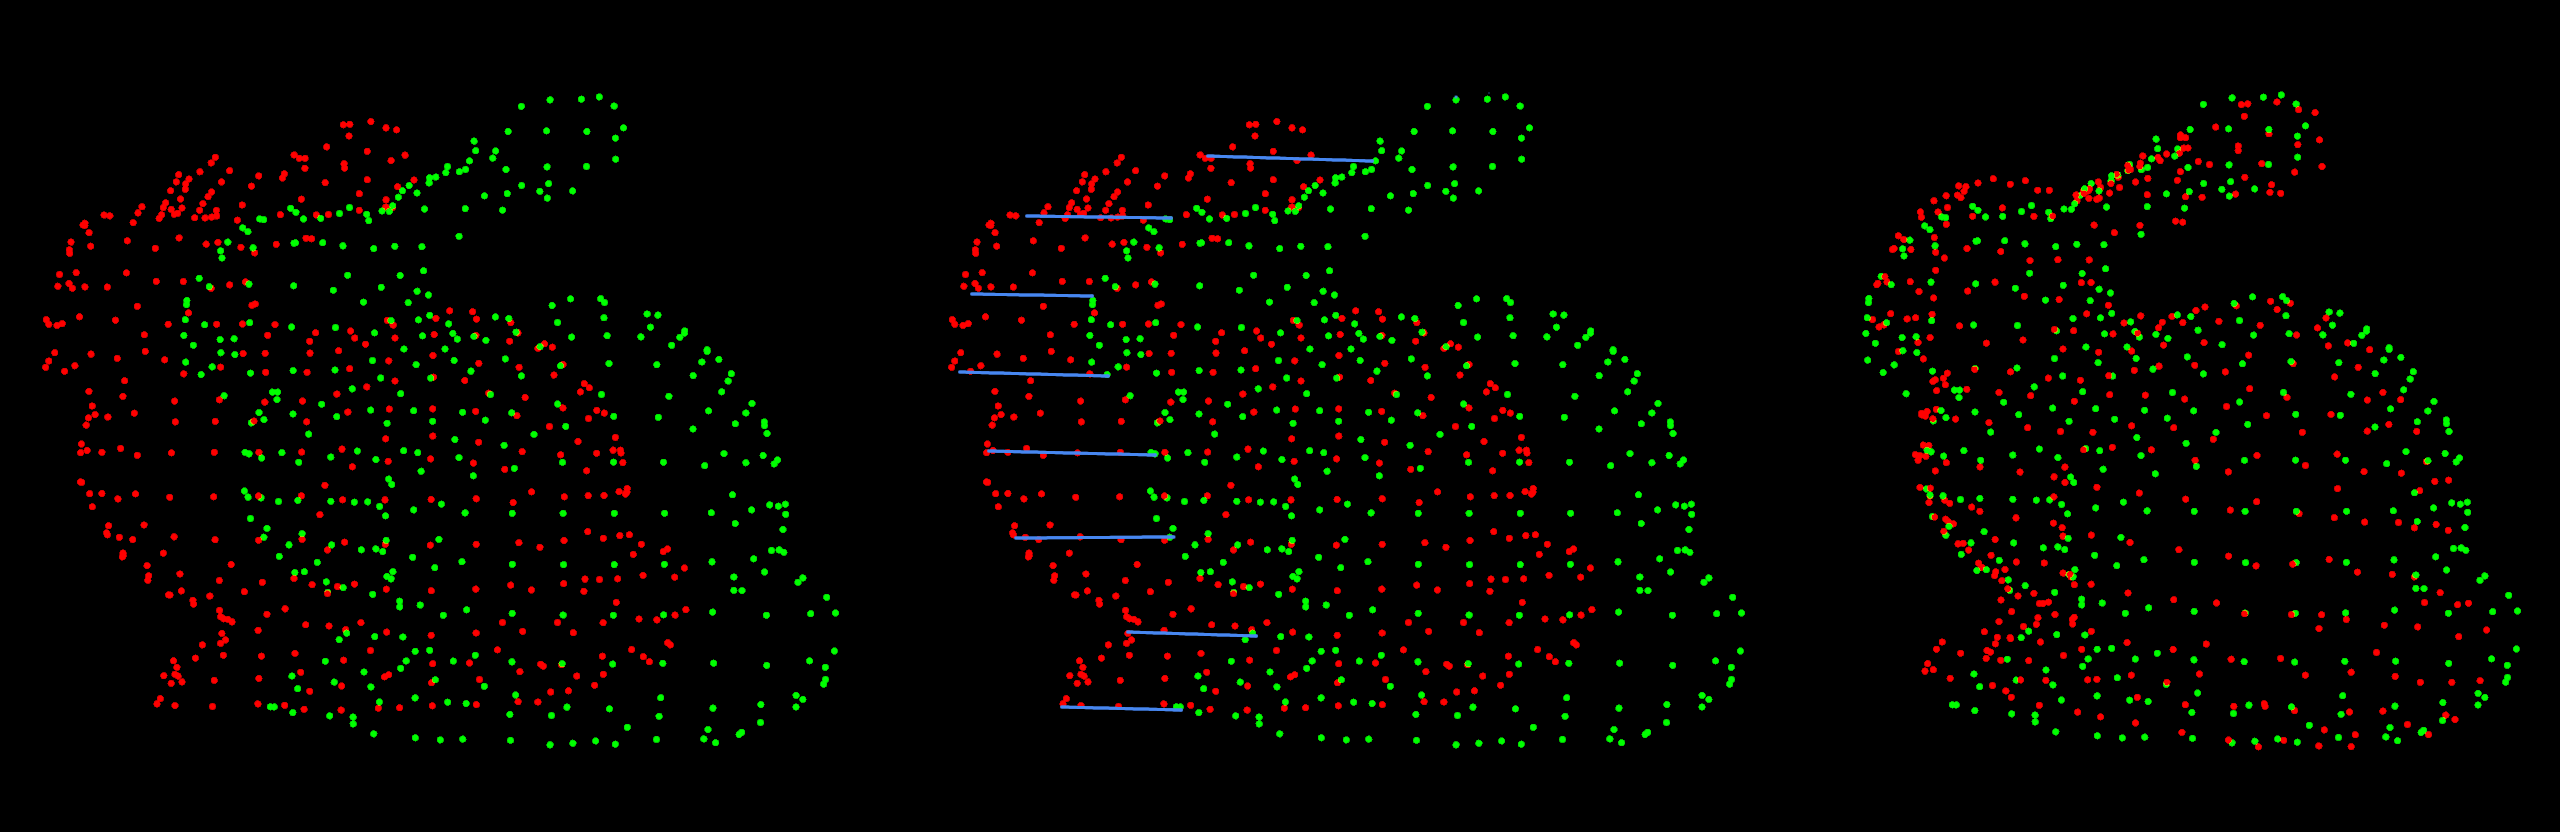
\includegraphics[scale=0.15]{registration_bunny}
\caption{Ejemplo de alineamiento de dos nubes de puntos.}\label{fig:registration_bunny}
\end{figure}


Para conocer en mayor detalle el proceso de alineamiento, se muestra en la figura \ref{fig:registration_flow} el conjunto de pasos que se siguen desde que se indican las nubes de entrada hasta que se obtiene la fusión de las mismas.

\begin{figure}
\centering
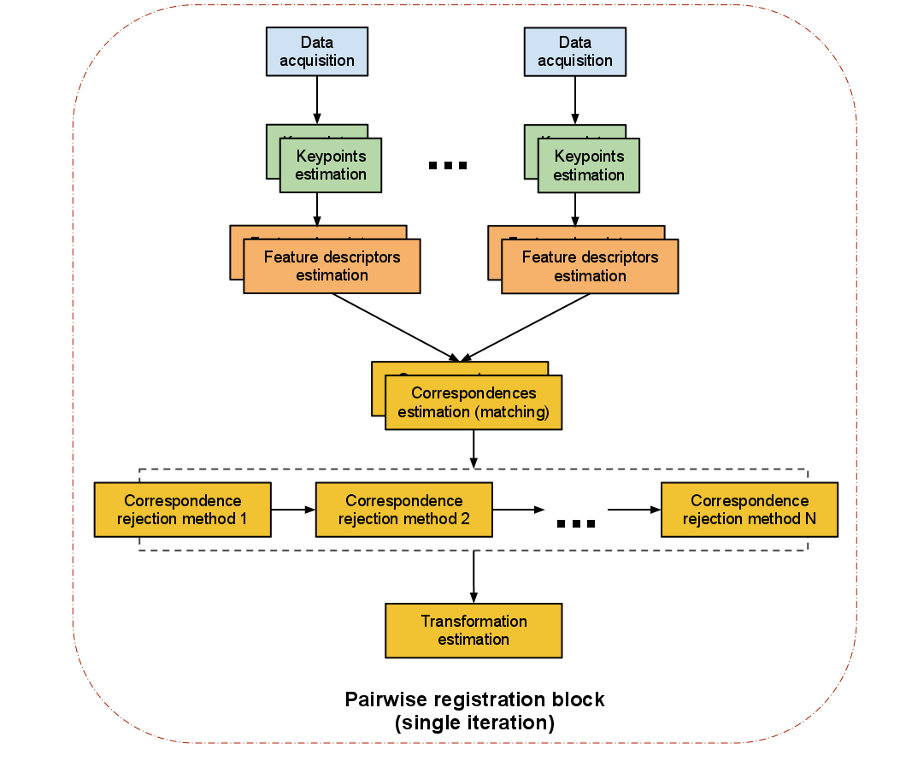
\includegraphics[scale=0.5]{registration_flow}
\caption{Procedimiento completo para llevar a cabo el alineamiento de nubes de puntos.}\label{fig:registration_flow}
\end{figure}


Dadas dos o más nubes de puntos como entrada, el primer paso implica extraer keypoints o puntos clave de cada una de ellas. Por keypoint, punto clave o punto de interés se entiende como un punto de la nube que representa características especiales de la misma tal y como son esquinas o bordes. Por lo tanto, las principales características de un keypoint pueden resumirse en los siguientes puntos:

%https://en.wikipedia.org/wiki/Interest_point_detection

\begin{itemize}
\item[•] Tiene una clara definición matemática.
\item[•] Tiene una clara definición de su posición en el espacio.
\item[•] El entorno local alrededor del keypoint es rico en información característica de la nube de modo que el uso del keypoint simplifica el uso de la nube.
\item[•] Es estable ante perturbaciones locales y globales tal y como cambios de iluminación y brillo de modo que las operaciones aplicadas sobre estos puntos tengan elevada repetibilidad.
\item[•] De forma opcional, el keypoint puede incluir un atributo de escala para poder aplicar operaciones sobre keypoints obtenidos de imágenes reales así como poder tolerar cambios de escala.
\end{itemize}

%COMPLETAR CON http://www.pointclouds.org/assets/uploads/cglibs13_features.pdf

Por ejemplo, las esquinas detectadas en una nube de puntos o imagen pueden considerarse puntos clave pues muestran información característica sobre las delimitaciones del objeto detectado tal y como se aprecia en la figura \ref{fig:corner_detection}

\begin{figure}
\centering
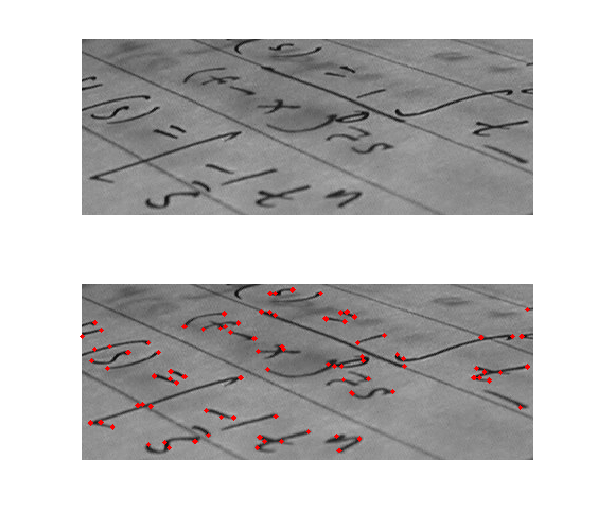
\includegraphics[scale=0.5]{corner_detection}
\caption{Ejemplo de detección de puntos clave en forma de esquinas.}\label{fig:corner_detection}
\end{figure}

Hasta el momento se ha hablado de puntos clave o keypoints de forma genérica sin embargo cabe destacar que existen diferentes tipos y es necesario especificar y definir cuál de ellos se va a utilizar de ahora en adelante.

Se puede considerar el harris keypoint o punto clave harris el cual ya se ha mencionado de forma indirecta en la figura \ref{fig:corner_detection} pues en realidad, ``harris'' hace referencia al método de extracción de esquinas y otras características utilizado en algoritmos de visión por computador. Fue introducido por Chris Harris y Mike Stephens en 1988.

Entrando ligeramente en detalle, una esquina puede definirse como un punto cuyo entorno toma dos direcciones dominantes y diferentes entre sí, es decir, una esquina es la intersección de dos bordes siendo un borde un cambio brusco del brillo en la imagen o en el caso, la nube de puntos. Por lo tanto, las esquinas son consideradas puntos de interés invariantes a la traslación, rotación y cambios de iluminación. 
Aunque las esquinas suponen una pequeña fracción de la nube, contienen la información más importante sobre la misma la cual se puede utilizar para labores de restauración de la nube o minimizar el tamaño o número de puntos.

No se darán detalles técnicos sobre los puntos de interés harris ya que en su lugar se va a trabajar con los puntos SIFT. 

Scale Invariant Feature Transform (SIFT) es un algoritmo utilizado en visión por computador para la extracción de características (features) locales en una imagen o nube de puntos. Las aplicaciones de este algoritmo son varias como reconocimiento de objetos, navegación, modelado 3D, reconocimiento de gestos o identificación de individuos.

Este algoritmo es de alta robustez y consistencia porque puede identificar objetos y características incluso en ambientes borrosos, confusos o sometidos a oclusión parcial porque se trata de un algoritmo invariante a cambios de escala, orientación, cambios de iluminación y parcialmente invariante a la distorsión afín, es decir, puede trabajar con partes de una nube de puntos cuya única diferencia es su orientación mientras que el resto de atributos permanecen idénticos.

Obtener correctamente los keypoints es de vital importancia ya que intentar alinear dos nubes considerando todos y cada uno de sus puntos puede suponer una carga computacional inconcebible para el caso de nubes de cientos de miles o incluso millones de puntos. 

el siguiente paso indicado en la figura \ref{fig:registration_flow} indica la estimación de los feature descriptors, es decir, los vectores donde se almacenan las características de la nube entorno a cada keypoint para poder compararlos entre sí. Por ejemplo se puede tener un vector que contiene normales a la superficie en cada keypoint o bien información sobre el brillo o luminosidad.

Una vez que se dispone de dos o más vectores de características, cada uno de una nube de puntos diferente, se pasa al siguiente paso en el que hay que encontrar la información equivalente entre vectores, es decir, las características de las nubes que pueden solaparse ya que son muy parecidas o idénticas. Dependiendo del tipo de característica que se quiera alinear o unificar existen diferentes métodos para encontrar correspondencias:

Para hacer coincidir puntos utilizando solamente sus coordenadas XYZ existen métodos tanto para nubes organizadas como desorganizadas:
\begin{itemize}
\item[•]Emparejamiento por fuerza bruta.
\item[•]Búsqueda del vecino más cercano mediante la librería FLANN.
\end{itemize}
en sus modalidades de:
\begin{itemize}
\item[•]Búsqueda directa de puntos en una nube organizada.
\item[•]Búsqueda en los índices de los puntos de una nube organizada.
\end{itemize}

Para la coincidencia de características diferentes a la posición de los puntos se tienen los siguientes métodos: 
\begin{itemize}
\item[•]Emparejamiento por fuerza bruta
\item[•]Búsqueda del vecino más cercano mediante la librería FLANN
\end{itemize}
en sus modalidades de:
\begin{itemize}
\item[•]Método de correspondencia directa (por defecto) Busca correspondencias en la nube modelo para todos y cada uno de los puntos de la nube fuente.
\item[•]Método de correspondencia recíproca con el que se buscan similitudes a la nube modelo en la nube fuente y viceversa quedándose solamente con la intersección.
\end{itemize}

No todas las correspondencias establecidas son correctas o de utilidad y es por esto por lo que hay que hacer una criba en el siguiente paso ya que las correspondencias inadecuadas pueden afectar negativamente a la transformación final. Para ello simplemente se puede utilizar una fracción del número total de correspondencias encontradas o utilizar algunos criterios de rechazo de correspondencias como los siguientes:

\begin{itemize}
\item[•]Rechazo basado en la \textbf{distancia}:
Se filtran correspondencias de la nube fuente si están a una distancia mayor que un valor determinado de su punto equivalente en la nube objetivo.
\item[•]Rechazo basado en \textbf{compatibilidad de normales}:
Utilizando la información sobre las normales en cada punto, se rechazan correspondencias con vectores normales inconsistentes, es decir, si el ángulo entre la normal en el punto de la nube fuente y la normal en su punto equivalente en la nube objetivo supera cierto valor.
\item[•]Rechazo basado en \textbf{correspondencias múltiples}: 
Varios puntos de la nube de entrada se corresponden con un único punto de la nube modelo. Para paliar esta situación, se suele escoger el punto de la nube de entrada más cercano al punto correspondiente en el modelo.
\item[•]Rechazo basado en \textbf{solapamiento}:
La nube fuente y la nube objetivo tienen un solapamiento parcial, aparecen correspondencias en puntos límite o frontera de dicho solapamiento dando lugar a errores posteriores. Una vez detectadas, estas correspondencias son eliminadas. 
\end{itemize}

Estos criterios de criba de correspondencias pueden apreciarse visualmente en la figura \ref{fig:metodos_criba}

\begin{figure}
\centering
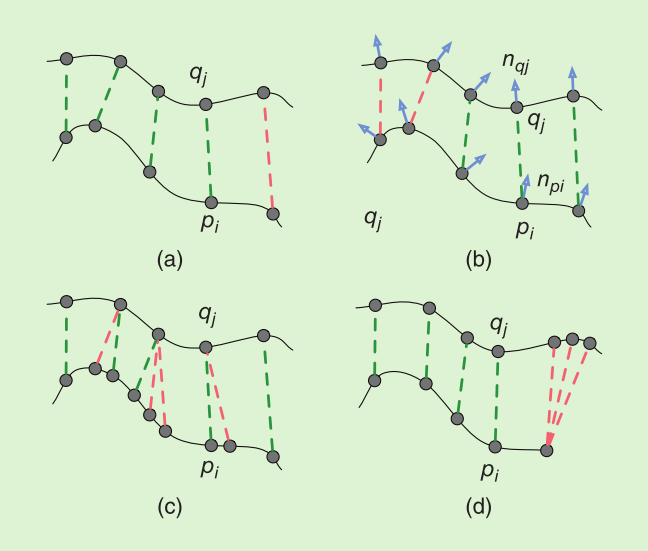
\includegraphics[scale=0.5]{metodos_criba}
\caption{Ejemplo de criba de correspondencias. Los puntos de la nube objetivo se representan como $q_j$ y los de la nube fuente como $p_i$. Se representan las técnicas de rechazo basado en la distancia (a), compatibilidad de normales (b), correspondencias múltiples (c) y solapamiento (d)}\label{fig:metodos_criba}
\end{figure}

En el último paso, se lleva a cabo la transformación de la nube fuente siguiendo estos puntos:

\begin{itemize}
\item[•]Evaluar el error existente entre los puntos de la nube fuente y sus equivalentes en la nube modelo (por ejemplo, la distancia que los separa cuando ambas nubes se representan en el mismo espacio)
\item[•]Estimar una transformación rígida de la nube fuente (es decir, conservando distancias y ángulos dentro de la misma nube) para minimizar el error evaluado anteriormente.
\item[•]Realizar la transformación de forma iterativa hasta converger a una solución aceptable.
\item[•]Optimizar la estructura de puntos resultante eliminando información redundante, por ejemplo.
\end{itemize}

Existen tres principales tipos de errores entre un punto de la nube fuente y su equivalente en la nube objetivo:

\begin{itemize}
\item[•]Error de distancia punto a punto:
Se trata de la distancia geométrica entre el punto de la nube fuente y su equivalente en la nube objetivo.

$$E_{punto\_punto}(T)=\sum_{k=1}^{N} w_{k}\| Tp_{k}-q_{k} \|^2$$

Donde $(p_{k},q_{k})$ es la $k-ésima$ de las $N$ correspondencias entre los puntos $p_k$ de la nube fuente y los puntos $q_k$ de la nube modelo. De forma opcional, se puede añadir un factor de peso $w_k$ para dar más o menos importancia a la correspondencia de puntos.

\item[•]Error de distancia punto a plano:
Es la distancia entre el punto de la nube fuente y el plano descrito por su punto equivalente junto a su vector normal en la nube objetivo.

$$E_{punto\_plano}(T)=\sum_{k=1}^{N} w_{k} ((Tp_{k}-q_{k})n_{qk}) ^2$$

Donde $n_{qk}$ es el vector normal al plano.

\item[•]Error generalizado:
Es una generalización de los dos tipos de errores anteriores. Utiliza las matrices de covarianzas de los entornos locales del punto de la nube fuente y su equivalente de la nube objetivo para alinear superficies en vez de puntos.

$$E_{generalizado}(T)=\sum_{k=1}^{N} {{d_{k}}^{(T)}}^{T} (\Sigma_{k}^{Q}+T\Sigma_{k}^{P}T^{T})^{-1}d_{k}^{(T)}$$

Donde $d_{k}^{(T)}=q_{k}-Tp_{k}$ son las distancias entre las correspondencias de los puntos $(p_{k},q_{k})$, $T$ es la matriz de transformación y $T^T$ es su traspuesta. Además, se hace uso de las matrices de covarianzas de todos los puntos en la nube fuente $P$ y objetivo $Q$ que son respectivamente $\Sigma_{k}^{P}$ y $\Sigma_{k}^{Q}$.

\end{itemize}

Se pueden visualizar este tipo de errores en la figura \ref{fig:tipos_errores} 

\begin{figure}
\centering
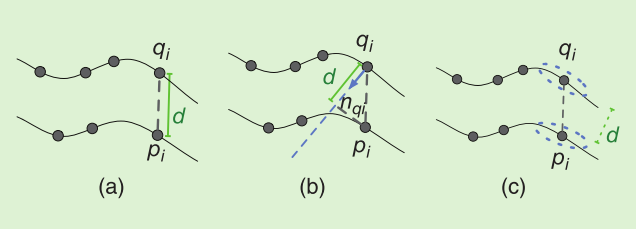
\includegraphics[scale=0.5]{tipos_errores}
\caption{Tipos de errores entre punto fuente y punto objetivo. Error de distancia punto a punto (a), error de distnacia punto a plano (b) y error generalizado (c)}\label{fig:tipos_errores}
\end{figure}

Se han mencionado los términos ``iterativa'' y ``converger'' y es que la transformación de la nube fuente hasta llegar a parecerse la máximo posible a la nube modelo no es única, se lleva a cabo un proceso iterativo. 

Sean dos nubes de puntos $n-dimensionales$:

$$M=\left\lbrace m_{i} | m_{i} \in R^n,\;\;i=1,2,...,N_{m} \right\rbrace$$
$$F=\left\lbrace f_{j} | f_{j} \in R^n,\;\;i=1,2,...,N_{f} \right\rbrace$$

Dicha transformación puede definirse de la siguiente manera:

$$E(R,\Delta T)=\sum_{i=1}^{N_m} \sum_{j=1}^{N_f} w_{ij} \| m_{i}-(Rf_{j}+\Delta t)  \|^2$$


con $w_{ij}$ como el peso que determina la dureza de la transformación pues permite que haya transformación si $w_{ij}=1$ o la anula en el caso $w_{ij}=0$

Esta operación se repite una y otra vez hasta que se converge a una solución y para lo cual hay que establecer criterios como los siguientes:

\begin{itemize}
\item[•]Máximo número de iteraciones:
Se ajusta un valor de máximo número de iteraciones dependiendo de la complejidad de la nube. Si se supera dicho valor, significa que la operación de alineamiento diverge.
\item[•]Límite absoluto de transformación: 
La iteraciones se detienen cuando se alcanza un valor de transformación lo suficientemente diferente a la transformación inicial
\item[•]Límite relativo de transformación:
Indica la máxima diferencia entre una operación de transformación y la anterior. Si se supera dicho límite se detiene el proceso de transformación.
\item[•]Límite de iteraciones similares: 
Se establece un límite de iteraciones para las cuales la transformación realizada es muy similar, es decir, las operaciones de trasformación a penas efectúan cambios en la nube.
\item[•]Error de mínimos cuadrados relativo:
Este criterio es similar al de límite relativo de transformación pero utilizando el valor del error de mínimos cuadrados en vez de el de transformación.
\item[•]Error de mínimos cuadrados absoluto:
Este criterio es similar al de límite absoluto de transformación pero utilizando el valor del error de mínimos cuadrados en vez de el de transformación.
\end{itemize}

Se pueden visualizar estos criterios de convergencia en la figura \ref{fig:metodos_convergencia}

\begin{figure}
\centering
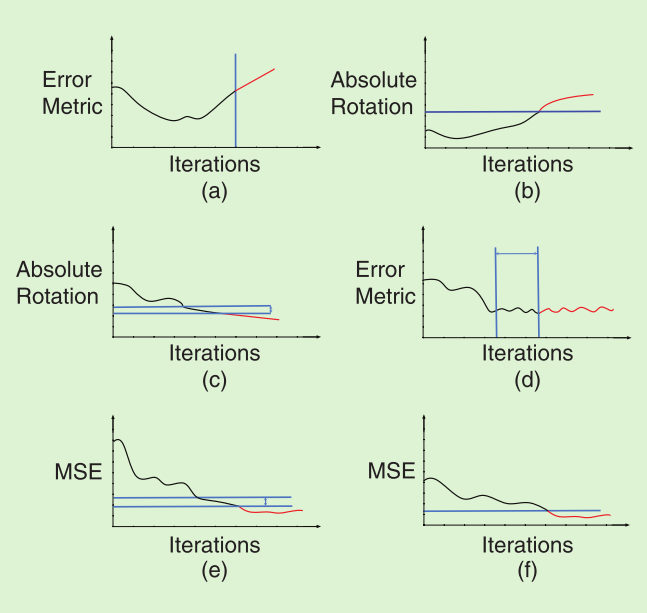
\includegraphics[scale=0.5]{metodos_convergencia}
\caption{Criterios de convergencia para la transformación iterativa. Máximo número de iteraciones (a), límite absoluto de tranformación (b), límite relativo de tranformación (c), límite de iteraciones similares (d), error de mínimos cuadrados relativo (e) y error de mínimos cuadrados absoluto (f). MSE significa Minimum Square Error, es decir, erro de mínimos cuadrados. }\label{fig:metodos_convergencia}
\end{figure}

%registration with the point cloud library ---> pdf
%https://en.wikipedia.org/wiki/Harris_Corner_Detector
%https://en.wikipedia.org/wiki/Scale-invariant_feature_transform


\section{Objetivos del TFG}
Una vez establecido el fundamento teórico relativo a las nubes de puntos en general y a la librería PCL se procede a continuación a exponer el motivo de este trabajo fin de grado.

Se tiene un doble objetivo que involucra por una parte la reproducción de algoritmos ya existentes y por otra la optimización de parte de los mismos.

La parte de reproducción de algoritmos existentes se refiere a desarrollar un programa escrito en C++ que sea capaz de extraer keypoints de una nube de puntos cualquiera siempre y cuando su formato sea PCD. Para ello se hace uso de la documentación ofrecida por la web oficial de PCL y los conocimientos propios de programación en C++. 

Habiendo desarrollado dicho programa, se procede a estudiar en detalle las partes de la librería PCL que utiliza, comprender cómo funcionan y medir tiempos de ejecución de los diferentes métodos nativos de PCL involucrados en todo el proceso de extracción de keypoints. De este modo, se detecta el algoritmo de mayor tiempo de ejecución y por lo tanto el de mayor carga computacional. Finalmente, se estudia la mencionada parte del código y se plantea cómo crear hardware digital exclusivamente para la optimización de la parte del código de PCL y no de las librerías adicionales en las que se apoya. Puesto que no todo tipo de software es sintetizable en hardware, deberán hacerse simplificaciones o incluso cambios sustanciales al código original para posibilitar su síntesis. Para llevar a cabo este proceso se utilizarán conocimientos de High Level Synthesis (HLS) que se traduce como síntesis de alto nivel y puede definirse como un proceso automatizado que interpreta una descripción algorítmica de un deseado comportamiento y crea hardware digital que implementa dicho comportamiento.

La plataforma sobre la que se comprobará la compleción de dichos objetivos es una FPGA cuyas características se exponen en el apartado \ref{herraminetas_hardware}

Como objetivo o punto adicional, se desarrolla también código en C++ para mostrar nubes de nubes de puntos por pantalla y así poder representar de una manera visual e intuitiva diferentes conjuntos de puntos y las operaciones efectuadas sobre los mismos. Es importante destacar que esta funcionalidad no funciona en la FPGA ya que no tiene soporte gráfico.



\section{Descripción e instalación de herramientas necesarias para desarrollar el trabajo}
Para realizar el presente trabajo se requieren herramientas que pueden clasificarse en dos tipos: software y hardware.
\subsection{Herramientas hardware} \label{herraminetas_hardware}
La principal herramienta hardware de la que se dispone y sobre la cual se comprobarán los resultados de la aplicación de los objetivos del presente trabajo es una Pynq-Z1\cite{pynq}. 

Se trata del soporte hardware para la tecnología PYNQ que es de libre uso. Ésta permite explotar las capacidades de los sistemas en chip programables sin tener que diseñar circuitos de lógica programable la cual ya ha sido diseñada usando Python. De este modo, los circuitos de lógica programable son importados como librerías hardware y configurados según sus APIs de la mism aforma que las librerías software son importadas y configuradas.

Algunas de las características principales de la Pynq-Z1 son:

\begin{itemize}
\item[•] Un procesador Cortex-A9 de dos núcleos a 650MHz
\item[•] Controlador de memoria DDR3 con 8 canales DMA y 4 puertos esclavos AXI3 de alto rendimiento
\item[•] Periféricos con elevado ancho de banda: Ethernet 1G, USB 2.0 y SDIO 
\item[•] Controlador de periféricos de gran ancho de banda: SPI, UART, CAN, I2C
\item[•] 630KB de memoria RAM
\item[•] Programable con JTAG, flash Quad-SPI y tarjeta micro SD
\end{itemize}




\subsection{Herramientas software}
\subsubsection{Máquina virtual}
La principal herramienta software utilizada para el desarrollo del TFG se trata de una máquina virtual. Esto se debe a que las computadoras con las que se realiza el trabajo, ya sean las disponibles en el laboratorio del CEI o el computador personal del autor, corren con un sistema operativo Windows. Por cuestiones de comodidad y sobre todo facilidad de instalación y desinstalación de software se opta por trabajar en un sistema operativo basado en linux, en concreto, las distribuciones ubuntu 18.04.1 64 bits para la computadora del autor y xubuntu 64 bits para las computadoras del laboratorio. Por lo tanto, a partir de este punto, salvo que se mencione lo contrario, el sistema de archivos e instrucciones ejecutadas por línea de comandos así como demás características propias de diferentes sistemas operativos se refieren a un sistema operativo basado en linux.

La máquina virtual se crea haciendo uso del software VirtualBox el cual facilita la creación y personalización de máquinas virtuales no solamente basadas en linux sino en cualquier otro sistema operativo.

%https://www.virtualbox.org/

\subsubsection{PCL}
Dicho lo cual, disponiendo ya de una máquina virtual, es necesario instalar las librerías de PCL. Para ello se visita la web oficial de PCL pues ésta ofrece las instrucciones adecuadas. Para poder instalar PCL en linux se deben ejecutar los siguientes comandos:

%http://pointclouds.org/downloads/

\begin{verbatim}
sudo add-apt-repository ppa:v-launchpad-jochen-sprickerhof-de/pcl
sudo apt-get update
sudo apt-get install libpcl-all
\end{verbatim}

La primera instrucción añade al sistema el repositorio en el que se encuentra la librería, el segundo busca actualizaciones disponibles y por último se procede a la instalación de todos los archivos actualizados.

Cuando la instalación está completa, se generan una serie de carpetas en el directorio /usr/include:

\begin{itemize}
\item[•]pcl-1.8: Es la versión 1.8 de la librería de PCL. Contiene en su interior la carpeta pcl que con todos los módulos de PCL estructurados correctamente.
\item[•]eigen3: Librería eigen que se encuentra bajo la carpeta Eigen dentro de este directorio.
\item[•]FLANN: Librería FLANN que se encuentra bajo la carpeta flann dentro de este directorio.
\item[•]vtk-x: versión x de la librería vtk 
\end{itemize}

\subsubsection{Vivado HLS}
Ya está instalado PCL en el sistema, ahora falta adquirir una herramienta adecuada para síntesis de software en hardware digital. Para ello se elige la herramienta vivado HLS de Xilinx. Accediendo a la web oficial de descargas se puede descargar la versión deseada de este software ya sea como un archivo comprimido TAR o un instalador web para mayor comodidad.

%https://www.xilinx.com/support/download.html
%https://www.xilinx.com/products/design-tools/vivado/integration/esl-design.html
\begin{figure}[!htb]
\centering
\minipage{0.8\textwidth}
  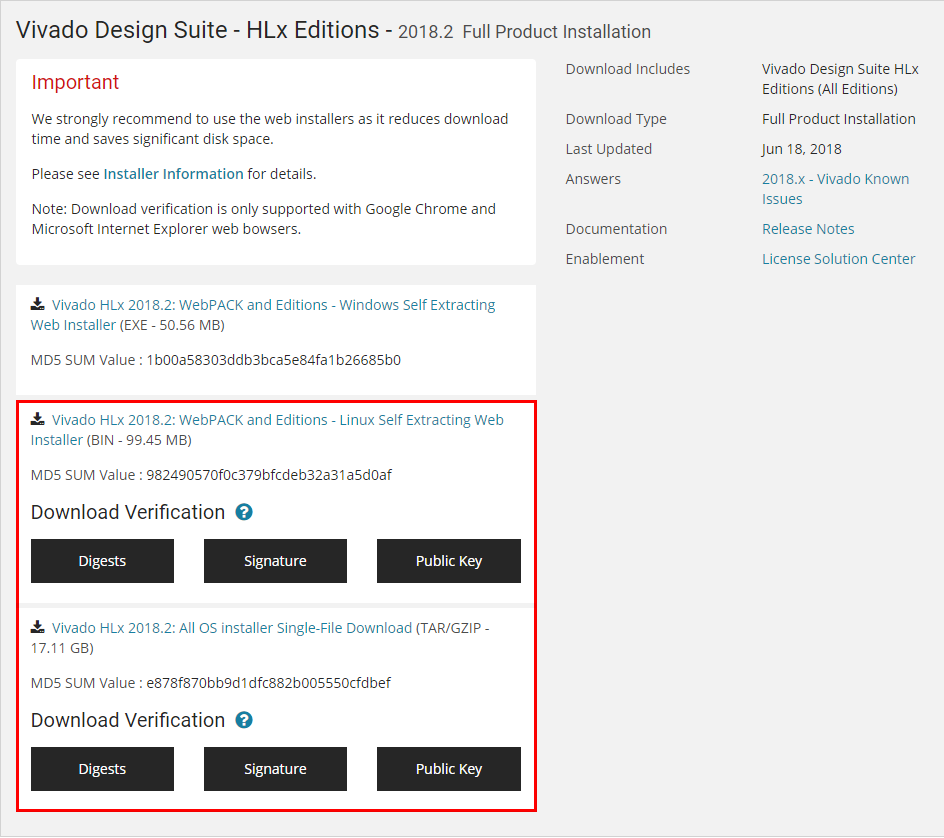
\includegraphics[width=\linewidth]{instalacion_xilinx_web}
  \caption{Selección de la versión 2018.2 para la instalación de Vivado}\label{fig:instalacion_xilinx_web}
\endminipage\hfill
\end{figure}

Durante el proceso de instalación...


Tras el proceso de instalación y habiendo otorgado los correspondientes permisos de licencia, se creará la carpeta Xilinx bajo el directorio /opt de forma que en /opt/Xilinx se pueden encontrar todas las herramientas que aporta este software.

Para poder utilizar la herramienta de Vivado HLS en linux se deben ejecutar los siguientes comandos:

\begin{verbatim}
source /opt/Xilinx/
vivado_hls
\end{verbatim}
El primero carga el archivo de configuración x en la sesión actual de la consola de comandos (hay que repetir este paso si se cierra la consola y se desea abrir de nuevo vivado hls)
\\
El segundo permite abrir el programa Vivado HLS para trabajar en la síntesis de hardware digital.



\section{Conclusiones}
Con el cierre del presente capítulo terminan las explicaciones fundamentales tanto de teoría como de herramientas que permiten estructurar el TFG.

En el siguiente capítulo se mostrarán las primeras tareas que giran entorno a la librería PCL para así poder visualizar nubes de puntos y extraer keypoints de las mismas.

